\Class{Gladiator}
{I might be a slave, but I am famous, I dine well, and my company is that of the finest noble women. Tell me, what do you have that I do not, slave trader---except the freedom to feel miserable?}{Jarek, arena champion}

The arena is the battlefield of the gladiator. From hand-to-hand combat in the mud pits of small forts to the grand games of the city-states, the gladiator is a warrior who fights to the sounds of people cheering his name or cursing his presence. A master of crowd control and the art of prolonged combat, gladiators are trained to fight.

They train to best wild beasts in deadly games for the amusement of the masses. They fight for glory, wealth, prestige and power. They fight to survive. Some are merely slaves, having to fight and perhaps hoping to win a chance to obtain freedom, while some fight willingly for the thrill of combat or the promise of riches and fame.

\WarriorTable[l l C C C p{8cm}]{The Gladiator}{
1 & +1 & +2 & +0 & +0 & Exotic weapon, gladiatorial performance, mercy, combat stance, martial display, team strike +1/+1d4\\
2 & +2 & +3 & +0 & +0 & Arena guile, Improved Unarmed Strike \\
3 & +3 & +3 & +1 & +1 & Improved Feint, taunt $-1$\\
4 & +4 & +4 & +1 & +1 & Uncanny dodge \\
5 & +5 & +4 & +1 & +1 & Armor optimization, exotic weapon \\
6 & +6/+1 & +5 & +2 & +2 & No mercy, shake off \\
7 & +7/+2 & +5 & +2 & +2 & Team strike +2/+2d4\\
8 & +8/+3 & +6 & +2 & +2 & Improved uncanny dodge, taunt $-2$ \\
9 & +9/+4 & +6 & +3 & +3 & Exotic weapon, trick \\
10 & +10/+5 & +7 & +3 & +3 & Armor optimization \\
11 & +11/+6/+1 & +7 & +3 & +3 &  \\
12 & +12/+7/+2 & +8 & +4 & +4 & Chant, combat stance (swift action), martial display (swift action) \\
13 & +13/+8/+3 & +8 & +4 & +4 & Exotic weapon, team strike +3/+3d4 \\
14 & +14/+9/+4 & +9 & +4 & +4 & Parry, taunt $-3$ \\
15 & +15/+10/+5 & +9 & +5 & +5 & Armor optimization, superior feint, threatening glare \\
16 & +16/+11/+6/+1 & +10 & +5 & +5 &  \\
17 & +17/+12/+7/+2 & +10 & +5 & +5 & Exotic weapon \\
18 & +18/+13/+8/+3 & +11 & +6 & +6 & Dragon's fury \\
19 & +19/+14/+9/+4 & +11 & +6 & +6 & Improved parry, team strike +4/+4d4 \\
20 & +20/+15/+10/+5 & +12 & +6 & +6 & Armor optimization, taunt $-4$}

\begin{figure}[t!]
\centering
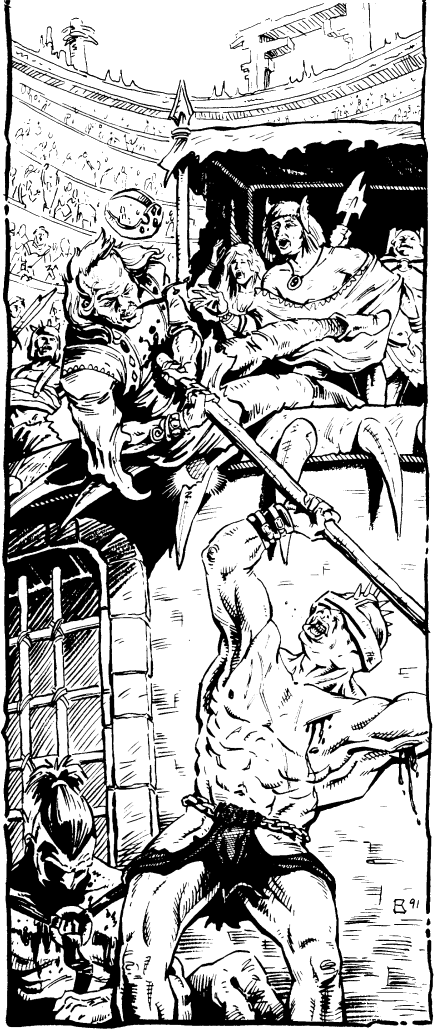
\includegraphics[width=\columnwidth]{images/arena-2.png}
\end{figure}

\subsection{Making a Gladiator}
Gladiators are among the best one-on-one fighters in all the Tablelands. They are trained in hand-to-hand combat before moving on to the use of exotic weapons of the arena. They learn to improvise weapons, wielding broken bones or wooden shafts with deadly precision. They learn how to taunt and tease opponents, driving them to reckless acts and taking advantage of the situation to strike down or maim a foe.

After all, a long, drawn-out combat is more a crowd pleaser than a ten-second bout.

\textbf{Abilities:} Strength and Constitution are vital to a gladiator, since he is often in harm's way. Intelligence is useful for gaining plenty of skills points, which a gladiator needs to purchase Bluff, Intimidate, Performance, and Sense Motive, key skills for any arena performer.

\textbf{Races:} All races of Athas can be found in the arenas of the Tablelands. Muls, with their mixed dwarven and human parentage, are highly prized in the arenas. They are often bought for a high price and treated well in return for victory on the combat floor. Elves are often used for their swiftness and natural flair for taunting their opponent. Humans are the most common of gladiators, since humans are the most common race in the Tablelands. Halflings make poor gladiators, since they abhor slavery and will usually starve themselves to death rather than being used as commodities by anyone. The savage races of the wastes are often used as gladiators, usually as fodder for the most successful gladiators, though those demonstrating excellent combat prowess receive formal training.

\textbf{Alignment:} Gladiators are of all alignments. Some gladiators will obey all arena rules, being lawful individuals, though these often do not last long in the arena. Many gladiators tend toward a chaotic alignment. Evil gladiators use dirty tricks to gain an advantage over an opponent. Gladiators of all alignments can become crowd favorites, increasing their chances of winning their matches, since often times these matches are prearranged. The intrigues of the city-states can reach deep into the arena.

\subsection{Game Rule Information}

\textbf{Hit Die:} d12.

\subsubsection{Class Skills}
\skill{Balance} (Dex), \skill{Bluff} (Cha), \skill{Climb} (Str), \skill{Craft} (Int), \skill{Intimidate} (Cha), \skill{Jump} (Str), \skill{Perform} (Cha), \skill{Profession} (Wis), \skill{Sense Motive} (Wis), \skill{Spot} (Wis), \skill{Tumble} (Dex).

\textbf{Skill Points per Level:} 4 + Int modifier ($\times4$ at 1st level).

\subsubsection{Class Features}

\textbf{Weapon and Armor Proficiency:} You are proficient with all simple and martial weapons, light armor, medium armor and shields (except tower shields).

\textbf{Gladiatorial Performance:} Once per day per gladiator level, you can use your talents to affect enemies and allies. Each ability requires both a minimum gladiator level and a minimum number of ranks in the \skill{Perform} skill to qualify.

Starting a gladiatorial performance effect is a standard action unless otherwise stated. Some effects require concentration, which means you must take a standard action each round to maintain the ability.

\textit{Combat Stance:} A gladiator with 3 or more ranks in \skill{Perform} can assume a combat stance, showing off to spectators and displaying a warning to opponents. You receive a +2 competence bonus to AC against the first attack made against you within 5 rounds after assuming the stance. Combat stance can be assumed as a move action. At 12th level, a gladiator can assume it as a swift action.

\textit{Martial Display:} A gladiator with 3 or more ranks in \skill{Perform} can entertain the crowd and intimidate enemies with a display of unarmed attacks or weapon prowess. You receive a +2 competence bonus to the first attack roll you make within 5 rounds after ending the martial display. Martial display can be assumed as a move action. At 12th level, a gladiator can use martial display as a swift action.

\textit{Team Strike:} A gladiator with 3 or more ranks in \skill{Perform} can distract an enemy so an ally can exploit a vital spot when making a melee attack. Team strike can only be used against an enemy you threaten with a melee weapon. The ally must act on the same initiative as you or before your next turn to gain the benefit of team strike. The ally receives a +1 bonus to hit and inflicts an additional 1d4 points of damage on the next melee attack against the target. If the enemy moves out of your threat range before your ally attacks, the ally does not receive the benefits of team strike. Creatures immune to sneak attack damage and critical hits are immune to team strike. At 7th level and every six levels thereafter these bonuses increase by +1 to attack and +1d4 to damage (+2 attack and +2d4 damage at 7th, +3 attack and +3d4 at 13th, +4 attack and +4d4 at 19th).

\textit{Taunt:} A gladiator of 3rd or higher level with 6 or more ranks in \skill{Perform} can demoralize enemies by verbal ridicule. Enemies must be within 9 meters of the gladiator and capable of hearing you, and you must be able to see your enemies. Each enemy affected suffers a $-1$ morale penalty to attack and damage rolls, and a $-1$ morale penalty on saving throws versus charm and fear effects. The effect lasts as long as enemies hear your taunts and for 5 rounds thereafter. At 8th level and every six gladiator levels thereafter, the penalties increase by 1 ($-2$ at 8th, $-3$ at 14th and $-4$ at 20th). Taunt is a mind-affecting ability.

\textit{Shake Off:} A gladiator of 6th or higher level with 9 or more ranks in \skill{Perform} can try to end a mind-affecting effect in play on himself or an ally. You shake your head violently to clear your mind, or slap an ally to bring her back to her senses. The recipient of the shake off can reroll a single failed save or opposed skill check (with the same DC as the failed roll) to end a mind-affecting effect. If there is no save or check to avoid the mind-affecting effect, the effect ends automatically.

\textit{Trick:} A gladiator of 9th or higher level with 12 or more ranks in \skill{Perform} can temporarily confuse an adversary through the use of ploy and deception. The creature to be tricked must be within 9 meters, able to see and hear you. You must also be able to see the creature. You make an opposed Bluff check (vs. Sense Motive) as a move action. If the creature succeeds on the opposed roll, you cannot attempt to trick that creature again for 24 hours. If its roll fails, the creature becomes dazed (unable to act, but can defend normally) for 1 round. For every three gladiator levels attained beyond 9th, you can target one additional creature with a single use of this ability (two at 12th level, three at 15th, four at 18th).

\textit{Chant:} A gladiator of 12th or higher level with 15 or more ranks in \skill{Perform} can start a chant. The chant boosts the gladiator or an ally's abilities, granting a +2 competence bonus to AC, skill checks and saving throws. To be affected an ally must be within 9 meters of you. For every three levels attained beyond 12th, you can affect one additional creature within 9 meters (two creatures at 15th level, three at 18th). Combat chant is a mind-affecting ability which lasts as long as you chant and for 5 rounds thereafter.

\textit{Threatening Glare:} A gladiator of 15th or higher with 18 or more ranks of \skill{Perform} can panic enemies with his mere gaze. Creatures within a 9 meters radius that can see you must make a Will Save (DC 10 + half your class level + your Charisma bonus). On failing, creatures with less HD than you are affected as if under the effects of a fear spell for 5 rounds. Those with equal to or more than your HD become shaken for 5 rounds. If the creature succeeds on the save you cannot attempt to affect that creature again for 24 hours. Threatening Glare is a mind-affecting gaze affect.

\textit{Dragon's Fury:} A gladiator of 18th or higher level with 21 or more ranks in \skill{Perform} can enter a trance-like state in which his full offensive gladiatorial potential is unleashed.

You are immune to fear effects, receive a +4 competence bonus to attack rolls and damage rolls, and an additional attack per round made at your highest base attack bonus. In addition, you gain two temporary hit points per class level. Dragon's fury lasts for 10 rounds.

\textbf{Mercy (Ex):} At 1st level, you suffer no penalty to attack rolls when attacking with a weapon to inflict nonlethal damage.

\textbf{Exotic Weapon:} At 1st, 5th, 9th, 13th, and 17th level, you receive \feat{Exotic Weapon Proficiency} as a bonus feat.

\textbf{Improved Unarmed Strike:} At 2nd level you \feat{Improved Unarmed Strike} as a bonus feat.

\textbf{Arena Guile (Ex):} Starting at 2nd level, you add one-half your gladiator level (round down) as a bonus to all \skill{Bluff} and \skill{Sense Motive} checks that relate directly to melee combat.

\textbf{Improved Feint:} You are adept at deceiving your opponents. At 3rd level, you gain \feat{Improved Feint} as a bonus feat.

\textbf{Uncanny Dodge (Ex):} At 4th level, you retain your Dexterity bonus to AC (if any) even if you are caught flat-footed or struck by an invisible attacker. However, you still lose your Dexterity bonus to AC if immobilized. If you already have uncanny dodge from a different class, you automatically gain improved uncanny dodge (see below) instead.

\textbf{Armor Optimization (Ex):} At 5th level, 10th, 15th, and 20th level, choose one of the following benefits which applies whenever you are wearing any armor you are proficient with:

\begin{itemize*}
\item +1 bonus to AC.
\item $-1$ armor check penalty.
\item +1 maximum Dexterity bonus.
\item Armor is treated as one category lighter (e.g. medium armor is treated as light armor).
\end{itemize*}

Each time this feature is gained, you must choose a different benefit.

\textbf{No Mercy (Ex):} Beginning at 6th level, you can perform a coup de grace as a standard action rather than a full-round action.

\textbf{Improved Uncanny Dodge (Ex):} At 8th level and higher, you can no longer be flanked. This defense denies a rogue the ability to sneak attack you by flanking you, unless the attacker has at least four more rogue levels than you have gladiator levels. If you already have uncanny dodge (see above) from a second class, the levels from all classes that grant uncanny dodge stack to determine the minimum level a rogue must be to flank you.

\textbf{Parry (Ex):} Beginning at 14th level, once per round you can forfeit an attack to attempt to parry an incoming melee attack. The forfeited attack has to be the one with your highest base attack bonus. If wielding two weapons, the parry must be made using your primary weapon. You make an opposed attack roll with a $-5$ penalty against your attacker roll. If you succeed, the attack is parried and you suffer no damage or ill effects related to the attack, including touch attacks used to deliver spells.

\textbf{Superior Feint:} Beginning at 15th level, you can make a Bluff check to feint in combat as a free action, but only once per round.

\textbf{Improved Parry:} As parry (see above), except you no longer suffer a $-5$ penalty to your opposed attack roll.

\subsection{Playing a Gladiator}
Mastering the techniques of blade and shield is important to you, but even more is the sense of daring, danger, and even joy that you feel when you battle inside the arena. You fight for the glory, the thrill of combat, and for the adoration of the crowd. Thus, you approach each encounter as if the bards will sing of it for ages. Silver and concubines are pleasant tokens, but the real measure of your success is how loud the crowd screams your name when you step into the pit.

As a gladiator, you find adventure wherever an opportunity for glory exists. You might be one of the gladiators that went out of job when the sorcerer-king of you city was killed by Tyrians and now you have become a mercenary warrior, still looking for the thrill of combat. You might have been able to flee from your owner and now user your sword to protect your slave tribe.

\subsubsection{Religion}
Gladiators have no special religion of their own. Some may worship the sorcerer-king of the city-state they are in, while some few may worship the elemental forces. Often, the hard life of training and combat leaves the gladiator with little to think of except survival.

\subsubsection{Other Classes}
Gladiators tend to think of themselves as the superior warriors of the Tablelands, sometimes to the point of arrogance.

In a sense, though, they are right. Gladiators receive training in one-on-one combat, and the use of anything they can find as a weapon. However, a group of trained fighters fighting in concert is certainly a match for a bunch of gladiators, who are unused to fighting in groups. Like most people of Athas, gladiators have a deep distrust of magic, and tend to shun wizards. They view clerics as nothing more than healers, people who put their faith in abstract things rather than a sharp blade.

\subsubsection{Combat}
You revel in melee. Your place is battling against hulking baazrags and wicked tembo, where you can hear the crowd cheering and chanting your name. You make good use of your various trick abilities to give yourself an important edge in combat. Consider taking feats such as Toughness to increase your ability to soak up damage and partially offset your lack of heavy armor. Choose feats that enhance your combat capabilities (such as Arena Clamor and Brutal Attack) or increase your acting skills (such as Persuasive and Skill Focus).

Feints, tricks, and deception play a very important role in arena combat, but don't forget that you don't just need to win, you need to win dramatically. Pretend to be more wounded than you really are. Wait for the right to deliver the final blow.

\subsubsection{Advancement}
Gladiators come from all walks of like. Perhaps you were fascinated with the illustrious life the famous gladiators live. Perhaps you lost your freedom when your village was raided or because of debt, needing to fight for your freedom.

Your race matters little; anyone with the drive to win glory through arena combat is a good candidate for gladiator training. Although not everyone is as suited for arena combat as a mul or half-giant, but with enough training anyone can become a talented, or at least interesting gladiator.

As you become more skilled, your most important decisions are which specialization path you will take. The most common specialty paths are the blind-fighter, jazst, and the montare. The blind fighters specialize in a unique form of gladiatorial combat, battling in complete darkness. Jazst are widely traveled theatrical performers in the Athasian arenas and are usually early warm-up acts that amuse the eager crowds. Montare are gladiators who fight in mounted combat, riding a single mount, driving chariots or sometimes even a mobile war machine.

\subsection{Starting Packages}
\subsubsection{The Blind-Fighter}
Dwarf Gladiator

\textbf{Ability Scores:} Str 15, Dex 10, Con 15, Int 8, Wis 14, Cha 10.

\textbf{Skills:} \skill{Bluff}, \skill{Listen}, \skill{Perform}, \skill{Sense Motive}, \skill{Tumble}.

\textbf{Languages:} Common, Dwarven.

\textbf{Feat:} \feat{Blind-Fight}.

\textbf{Weapons:} Thanak (2d6/$\times$3).

\textbf{Armor:} Scale mail (+4 AC).

\textbf{Gear:} Standard adventurer's kit.

\subsubsection{The Jazst}
Elf Gladiator

\textbf{Ability Scores:} Str 10, Dex 17, Con 10, Int 8, Wis 13, Cha 14.

\textbf{Skills:} \skill{Bluff}, \skill{Diplomacy}, \skill{Intimidate}, \skill{Perform}, \skill{Sense Motive}, \skill{Tumble}.

\textbf{Languages:} Common, Elven.

\textbf{Feat:} \feat{Skill Focus} (Perform).

\textbf{Weapons:} Elven longblade (1d8/18--20).

\textbf{Armor:} Leather armor (+2 AC).

\textbf{Gear:} Standard adventurer's kit.

\subsubsection{The Montare}
Mul Gladiator

\textbf{Ability Scores:} Str 14, Dex 15, Con 13, Int 8, Wis 12, Cha 10.

\textbf{Skills:} \skill{Bluff}, \skill{Handle Animal}, \skill{Intimidate}, \skill{Perform}, \skill{Ride}, \skill{Sense Motive}.

\textbf{Languages:} Common.

\textbf{Feat:} \feat{Mounted Combat}.

\textbf{Weapons:} Heartpick (1d8/$\times$4)

Composite shortbow with 20 arrows (1d6/$\times$3, 21 m).

\textbf{Armor:} Leather armor (+2 AC).

\textbf{Gear:} Standard adventurer's kit.

\subsection{Gladiators on Athas}
\Quote{I am Darsus. I will be closer to you in these next few days, which will be the last days of your miserable lives, than the mother who first brought you screaming into this world. I did not pay good money for your company, I paid it so I could profit from your deaths. And just as your mother was there at your beginning, so I shall be there at your end. And when you die, and die you shall, your journey to the Gray will be to the sound of clapping and cheering. Don't let me down, and I won't feed your corpses to the jhakars.}{Darsus, arena manager}

In a world with civilizations as harsh as those of Athas, only the most bloodthirsty sports can entertain the crowds enough to keep their attention from their miserable lot in life. The arenas provide such sport with the spilling of blood by mighty gladiators. The killing is a release for the crowd, symbolic of that which the citizens cannot perform themselves.

It is therefore no wonder that the best of the gladiators rise above the crowd, to become the popular heroes of the age. Their exploits are the stuff of legends. Children follow their progress avidly, some even going so far as to paint the walls of the cities with pictures of their favorites in defiance of the templars. Some gladiators achieve such a measure of fame that their reputation spreads far from their city-states, bringing citizens of outlying towns to the arenas to witness these masters at their craft.

\subsubsection{Daily Life}

A gladiator must train constantly to maintain his puissance. Thus, much of his day is spent swinging wooden weapons, doing basic calisthenics, tightrope walking, and attending dodging practice. While out adventuring, a gladiator often spends time at night on watch practicing his move and stretching.

Once he has reached a respectable level of accomplishment, a gladiator might seek sponsorship from nobles and templars. These patrons offer better training and housing in return for no less than 50\% of the free gladiator's earnings and the companionship of the gladiator.

\subsubsection{Notables}

Famous gladiators usually fall into two categories: active gladiators who still perform in the many arenas of Athas, and former gladiators. Among those who still practice it there is Nightmare, a Gulgan blind gladiator who wears a great helm in the shape of a nightmare beast. Sandsinger is renowned elven jazst, and an accomplished dancer in and out of the arena. The most famous ex-gladiator of all is the mul Rikus of Tyr (page 282), responsible not for the death of one sorcerer-king, but three.

\subsubsection{Organizations}

High-level gladiators often find sponsorship from the rich. Nobles and templars will pay well to get an aspiring gladiator into their gladiator stables. Those cities that allow free gladiators to enter the games often have gladiators without such ties.

\subsubsection{NPC Reactions}

Easily motivated by promises of silver, glory, and freedom (whichever the employer possesses a surplus at the moment), gladiators can lend excellent, efficient muscle to any party. Most people look on gladiators with awe. The exception is when dealing with rival gladiators and their fans, which usually view them with contempt and try to belittle their abilities, generally displaying indifferent to unfriendly attitudes.

\subsubsection{Gladiator Lore}

Characters with ranks in \skill{Knowledge} (local) can research gladiators to learn more about them. When a character makes a skill check, read or paraphrase the following, including the information from lower DCs.

\textbf{DC 10:} A gladiator is a fighter with delusions of grandeur! These showoffs think they can live forever in a bard's song!

\textbf{DC 15:} Gladiators are extremely resilient and tricky combatants, and they seem to know with all kinds of weapons with the same degree of expertise.

\textbf{DC 20:} Some gladiators achieve such prestigious reputations that their fame spreads all over the Tablelands.
